\documentclass[10pt]{article} 
\usepackage{amsfonts} 
\usepackage{tikz}
\usepackage{amssymb} 
\usepackage{ulem} 
\usepackage{graphicx} 
\usepackage{subcaption}
\usepackage{amsthm}
\usepackage{systeme}
\usepackage{amsmath}
\usepackage{stmaryrd}
\usepackage{mathrsfs}
\usepackage{mathtools}
\usepackage{enumitem}
\usepackage{booktabs}
\usepackage{xcolor}
\usepackage{listings}
\usepackage{multicol}
\usepackage[utf8]{inputenc}
\usepackage[left=2.5cm,right=2.5cm,top=2cm,bottom=2cm]{geometry}
\usepackage[T1]{fontenc}
\usepackage{bbold}
\usepackage{subfiles}
\usepackage{hyperref}
\usepackage{titlesec}
\usepackage{natbib}
\usepackage{chngcntr}
\usepackage{url}
\usepackage{float}
\usepackage{xcolor}
\hypersetup{
        colorlinks=true,
        linkcolor=black,
        urlcolor=red
}
\usepackage{tikz}
\usetikzlibrary{shapes.geometric}
\usepackage{pgfplots}
\pgfplotsset{compat=1.17}
\usepgfplotslibrary{groupplots}

\pgfplotsset{
  every axis/.append style={
    grid=major,
    grid style={dashed},
    legend style={font=\tiny, legend columns = 1},
    ylabel style={font=\scriptsize},
    xlabel style={font=\scriptsize},
    width=\linewidth
  },
  every axis plot/.append style={line width=1.2pt, line join=round},
  every axis legend/.append style={legend columns=1},
  %group/group size=3 by 1,
  every x tick label/.append style={font=\small, alias=XTick,inner xsep=0pt},
  every y tick label/.append style={font=\small, alias=XTick,inner xsep=0pt},
  every x tick scale label/.style={at=(XTick.base east),anchor=base west}
}


\definecolor{col1}{RGB}{36, 61, 93}
\definecolor{col2}{RGB}{77, 143, 145}
\definecolor{col3}{RGB}{228, 206, 135}
\definecolor{col4}{RGB}{186, 161, 22}
\definecolor{col5}{RGB}{45, 3, 59}
\definecolor{col6}{RGB}{193, 71, 233}
\definecolor{col7}{RGB}{126, 134, 255}
\definecolor{col8}{RGB}{85, 170, 255}

\definecolor{darkyellow}{rgb}{0.85, 0.65, 0} 

\tikzset{
  curve1/.style={col1, mark=*, solid}, 
  curve2/.style={col2, mark=x, solid}, 
  curve3/.style={col3, mark=*, densely dashed}, 
  curve4/.style={col4, mark=x, dashed},
  curve5/.style={col5, mark= o,solid},
  curve6/.style={col6},
  curve7/.style={col7},
  curve8/.style={col8},
  curve9/.style={col1, densely dotted},
  curve10/.style={col2, dotted},
  curve11/.style={col3, dashdotted},
  curve12/.style={col4, dashed},
  curve13/.style={col5, dotted},
}

\setcitestyle{square, comma, numbers,sort&compress, super}
\setcounter{secnumdepth}{4}



\newcommand{\equivclass}[1]{%
  #1/{\sim}%
}

\newcommand{\veps}{\varepsilon}
\newcommand{\sqeps}{\square_{\varepsilon}}
\newcommand{\sqteps}{\square_{2\varepsilon}}
\newcommand{\hf}{\hat{f}}
\newcommand{\hg}{\hat{g}}
\newcommand{\R}{\mathbb{R}}
\newcommand{\Rd}{\mathbb{R}^{d}}
\newcommand{\Sd}{\mathbb{S}^{d-1}}
\newcommand{\W}{W_2^2}
\newcommand{\SW}{SW_2^2}
\newcommand{\sigk}{\sigma(k)}
\newcommand{\tauk}{\tau(k)}
\newcommand{\pit}{\pi_{\theta}}
\newcommand{\pmu}{\pit \# \mu}
\newcommand{\pnu}{\pit \# \nu}
\newcommand{\sigtheta}{\sigma_{\theta}}
\newcommand{\tautheta}{\tau_{\theta}}
\newcommand{\sigthetK}{\sigtheta(k)}
\newcommand{\tauthetK}{\tautheta(k)}
\newcommand{\Thetmui}{\Theta_{i}^{\mu}}
\newcommand{\Thetnui}{\Theta_{i}^{\nu}}
\newcommand{\Umui}{U_{i}^{\mu}}
\newcommand{\Unui}{U_{i}^{\nu}}
\newcommand{\Unuj}{U_{j}^{\nu}}
\newcommand{\sigi}{\sigma_i}
\newcommand{\taui}{\tau_i}
\newcommand{\sigik}{\sigi(k)}
\newcommand{\tauik}{\taui(k)}
\newcommand{\gradF}{\nabla f}
\newcommand{\Nstar}{\mathbb{N}^*}
\newcommand{\std}{\mathbb{\sigma}}
\newcommand{\N}{\mathbb{N}}
\newcommand{\lambdim}{\lambda^{\otimes d}}
\newcommand{\Lap}{\Delta}
\newcommand{\RanP}{\hat{P}}
\newcommand{\Ranu}{\hat{u}}
\newcommand{\keanu}[1]{\textcolor{black}{#1}}
\newcommand{\keanunew}[1]{\textcolor{black}{#1}}
\newcommand{\keanureview}[1]{\textcolor{black}{#1}}
\newcommand{\julie}[1]{\textcolor{black}{#1}}
\newcommand{\julien}[1]{\textcolor{black}{#1}}
\newcommand{\Zq}{\mathbb{Z}/2\mathbb{Z}}
\newcommand{\sd}{s_{d-1}}
\newcommand{\tcos}{\text{cos}}
\newcommand{\tsin}{\text{sin}}
\newcommand{\tacos}{\text{arccos}}
\newcommand{\tdet}{\text{det}}
\newcommand{\tspan}{\text{Span}}
\newcommand{\Haus}{\mathcal{H}_{d-1}}
\newcommand{\SWsq}{SW_{2}^{4}}
\newcommand{\indices}{\{1,\hdots,d\}}
\newcommand{\Lad}{\mathcal{L}}
\newcommand{\Ld}{\Lad^d}
\newcommand{\M}{\mathcal{M}}
\newcommand{\subf}{f_{-\infty}^{-1}}
\newcommand{\I}{\mathcal{I}}
\newcommand{\C}{\mathbb{C}_{d,2}}


\DeclareMathOperator*{\argmax}{arg\,max}
\DeclareMathOperator*{\argmin}{arg\,min}

\newtheoremstyle{theoremstyle}
    {\topsep}            
    {\topsep}        
    {}                  
    {}             
    {\bfseries}            
    { :}                     
    {.5em}                 
    {}  
\theoremstyle{theoremstyle}
\newtheorem{D}{Definition}
\newtheorem{Ds}{Definitions}
\newtheorem{Th}{Theorem}
\newtheorem{Lem}{Lemma}
\newtheorem{Prop}{Proposition}
\newtheorem{Props}{Propositions}
\newtheorem{Rk}{Remark}
\newtheorem{Ill}{Illustration}
\newtheorem{Cor}{Corollary}
\newtheorem{Obs}{Observation}



\definecolor{customgreen}{rgb}{0.156, 0.706, 0.239} 


\counterwithin{figure}{section}
 
\title{A User's Guide to Sampling Strategies for Sliced Optimal Transport}


\author{Keanu SISOUK \\ Keanu.Sisouk@lip6.fr \\
      CNRS, LIP6\\
      Sorbonne University
      \and
      Julie Delon \\julie.delon@u-paris.fr \\
      CNRS, MAP5\\
      Paris Cite University
      \and
      Julien Tierny \\ julien.tierny@sorbonne-universite.fr\\
      CNRS, LIP6 \\
      Sorbonne University\\
     	}



\newcommand{\fix}{\marginpar{FIX}}
\newcommand{\new}{\marginpar{NEW}}



\renewcommand{\figureautorefname}{Fig.~}
\renewcommand{\equationautorefname}{Eq.~}

\renewcommand{\sectionautorefname}{Sec.~}
\renewcommand{\subsectionautorefname}{Sec.~}
\renewcommand{\subsubsectionautorefname}{Sec.~}
\renewcommand{\tableautorefname}{Tab.~}
\date{}

\begin{document}
\maketitle

\begin{abstract}

This paper serves as a user's guide to sampling strategies for sliced optimal transport ~\cite{Rabin_texture_mixing_sw,bonneel2015sliced}. 
We provide reminders and additional regularity results on the Sliced Wasserstein distance.
We detail the construction methods, generation time complexity, theoretical guarantees, and conditions for each strategy. Additionally, we provide insights into their suitability for sliced optimal transport in theory. Extensive experiments on both simulated and real-world data offer a representative comparison of the strategies, culminating in practical recommendations for their best usage.

\end{abstract}


\section{Introduction}
\label{sec:intro}

\begin{figure*}[tb]
    \centering
    \includegraphics[width=0.848\linewidth]{figs/circuitnn.pdf} 
    \caption{Illustration of differentiable CircuitNN. CircuitNN is designed based on differentiable NAND gates. After DAS is guided by PI and PO pairs of the truth table, CircuitNN can get the precise circuit architecture logic equivalent to the truth table.}
    \label{fig:circuitnn}
\end{figure*}

% 1. Describe the importance of logic synthesis
% 2. Existing Problems
% (a) Neural Architecture Search: Unstable, Predefined Setting, etc.
% (b) Circuit Generation: Probabilistic Model, Logic Equivalence

With the rapid advancement of technology, the scale of integrated circuits (ICs) has expanded exponentially. 
This expansion has introduced significant challenges in chip manufacturing, particularly concerning power and area metrics.
A primary objective in IC design is achieving the same circuit function with fewer transistors, thereby reducing power usage and area occupancy.

Logic synthesis~\cite{hachtel2005logicsynth}, a critical step in electronic design automation (EDA), transforms behavioral-level circuit designs into optimized gate-level circuits, ultimately yielding the final IC layout. 
The primary goal of logic synthesis is to identify the physical implementation with the fewest gates for a given circuit function. 
This task constitutes a challenging NP-hard combinatorial optimization problem. 
Current logic synthesis tools~\cite{brayton2010abc, wolf2013yosys} rely on human-designed heuristics, often leading to sub-optimal outcomes.

Differentiable architecture search (DAS) techniques~\cite{liu2018darts, chu2020darts} offer novel perspectives on addressing challenges in this problem.
Circuit functions can be represented through truth tables, which map binary inputs to their corresponding outputs. 
Truth tables provide a precise representation of input-output relationships, ensuring the design of functionally equivalent circuits.
Inspired by this, researchers~\cite{deepmind2024ai4sys, wang2024tnet} have begun exploring the application of DAS to synthesize circuits directly from truth tables.
Specifically, \citet{deepmind2024ai4sys} proposed CircuitNN, a framework that learns differentiable connection structures with logic gates, enabling the automatic generation of logic circuits from truth tables.
This approach significantly reduces the complexity of traditional circuit generation. 
Building on this, \citet{wang2024tnet} introduced T-Net, a triangle-shaped variant of CircuitNN, incorporating regularization techniques to enhance the efficiency of DAS.

Despite these advancements, several challenges remain. 
The computational complexity of DAS grows quadratically with the number of gates, posing scalability issues.
Although triangle-shaped architecture~\cite{wang2024tnet} partially mitigates this problem, redundancy persists. 
%Additionally, DAS is susceptible to converging to local optima, limiting the ability to search architectures that satisfy the given truth tables~\cite{liu2018darts}. 
%Furthermore, hyperparameters (network depth and layer width) require extensive searches, introducing complexity and prolonging the synthesis process. 
Additionally, DAS is susceptible to converging to local optima~\cite{liu2018darts} and hyperparameters (network depth and layer width) require extensive searches. 
The challenges arise from the vast search space in DAS. 
% Even with predefined settings for CircuitNN, finding a configuration that meets the truth table requires extensive trial and error during the DAS process. 
Intuitively, limiting the search space through predefined parameters (network depth, gates per layer, and connection probabilities) can significantly reduce the complexity.

Recent advances~\cite{openai2023gpt4, abramson2024alphafold3, esser2024sd3, li2024mar} in conditional generative models have demonstrated remarkable performance across language, vision, and graph generation tasks. 
Motivated by these developments, we propose a novel approach to circuit generation that generates preliminary circuit structures to guide DAS in generating refined circuits matching specified truth tables. 
Firstly, we introduce CircuitVQ, a tokenizer with a discrete codebook for circuit tokenization. 
Built upon our Circuit AutoEncoder framework~\cite{hou2022graphmae,li2023maskgae,wu2025mgvga}, CircuitVQ is trained through a circuit reconstruction task. 
Specifically, the CircuitVQ encoder encodes input circuits into discrete tokens using a learnable codebook, while the decoder reconstructs the circuit adjacency matrix based on these tokens.
Subsequently, the CircuitVQ encoder serves as a circuit tokenizer for CircuitAR pretraining, which employs a masked autoregressive modeling paradigm~\cite{chang2022maskgit, li2023mage}. 
In this process, the discrete codes function as supervision signals. 
After training, CircuitAR can generate discrete tokens progressively, which can be decoded into initial circuit structures by the decoder of the CircuitVQ. 
These prior insights can guide DAS in producing refined circuits that match the target truth tables precisely.

Our key contributions can be summarized as follows:
\begin{itemize}
\item We introduce CircuitVQ, a circuit tokenizer that facilitates graph autoregressive modeling for circuit generation, based on our Circuit AutoEncoder framework;
\item Develop CircuitAR, a model trained using masked autoregressive modeling, which generates initial circuit structures conditioned on given truth tables;
\item Propose a refinement framework that integrates differentiable architecture search to produce functionally equivalent circuits guided by target truth tables;
\item Comprehensive experiments demonstrating the scalability and capability emergence of our CircuitAR and the superior performance of the proposed circuit generation approach.
\end{itemize}

% Motivation
% (a) Diffusion (Vision, Graph), Autoregressive (Language, Vision)
% (b) Circuit Generation for Predefined Setting
% (c) Neural Architecture Search for Strict Logic Equivalence

% Contribution
% (a) Circuit Tokenizer (new transformer arch, training strategy)
% (b) CircuitAR (train and gen strategies, post-ar strategy)
% (c) Extensive Evaluation including BitD (Bit Distance) for Scalability




\section{Reminders on the Sliced Wasserstein Distance} \label{sec:reminderSW}


%\subsection{Notations}


%{We write $\Sigma_N$ the set of permutations of $\llbracket 1,N\rrbracket$, and for $A$ an ensemble $|A|$ denotes its cardinal.}

%{For a prime integer $b$, $+_{\mathbb{Z}/b\mathbb{Z}}$ will denote the inner law of the group $\mathbb{Z}/b\mathbb{Z}$.}

\subsection{Definition}\label{sec:def}
{In the following, we write $\langle \cdot \ | \ \cdot \rangle$ the Euclidean inner product in $\Rd$, $\|\cdot\|$ the induced norm, $\Sd = \{ x\in \Rd \ |\ \|x\| = 1\}$ the unit
sphere of $\R^d$.}
{For $\theta\in\Sd$, we write $\pit:\Rd
\rightarrow \R$ the map $x \mapsto \langle \theta|x \rangle$,
$\sd$ the uniform measure over $\Sd$. %and $\mathcal{U}(\Sd)$ the uniform distribution of $\Sd$. 
We also denote $\#$ the push-forward
operation}~\footnote{The push-forward of a measure  $\mu$ on $\R^d$ by
  an application $T: \R^d \rightarrow \R^k$ is defined as a measure
  $T\#\mu$ on $\R^k$ such that for all Borel sets $B \in
  \mathcal{B}(\R^k), T\#\mu(B) = \mu(T^{-1}(B))$.}.

For two probability measures $\mu$ and
$\nu$ supported in $\R^d$ {and with finite moments of order 2}, the Sliced Wasserstein
Distance between  $\mu$ and
$\nu$ is defined as
\begin{equation} \label{eq:SW}
\SW(\mu,\nu)= \mathbb{E}_{\theta \sim \mathcal{U}(\Sd)}[\W(\pmu, \pnu)] = \displaystyle\int_{\Sd}\W(\pmu, \pnu) d\sd(\theta).
\end{equation}

This distance, introduced
in~\citep{Rabin_texture_mixing_sw},  has been thoroughly studied and
used as a dissimilarity measure between probability distributions in machine
learning~\citep{bonneel2015sliced,nadjahi2021sliced,kolouri2018slicedAE},
and more generally as an alternative to the Wasserstein distance. % leveraging the simplicity of computing such distances in one dimension.
Its simplicity stems from the fact that the
Wasserstein distance between two probability measures in one dimension has
an explicit formula. Indeed, for two probability
measures $\rho_1$ and $\rho_2 $ on the line, the Wasserstein distance   $W_2(\rho_1,\rho_2)$ can be written
\begin{equation}
\label{eq:transport_ligne}
 W_2^2(\rho_1,\rho_2) =  \int_0^1 |F_1^{-1}(t)- F_2^{-1}(t)|^2dt,
\end{equation}
where  $F_1$ and $F_2$ are the cumulative distribution
functions of $\rho_1$ and $\rho_2 $, and $F_1^{-1}$ and $F_2^{-1}$ are
their respective
generalized inverses (see~\citep{santambrogio2015optimal} Proposition
2.17).  For two one dimensional discrete measures $\rho_1 =
\frac{1}{N}\sum\limits_{k=1}^N \delta_{x_k}$ and  $\rho_2 =
\frac{1}{N}\sum\limits_{k=1}^N \delta_{y_k}$, this distance becomes
\begin{equation}\label{eq:transport_ligne_2D_disc}
W_2^2(\rho_1,\rho_2) = \frac 1 N \sum_{k=1}^N |x_{\sigma(k)} -
y_{\tau(k)}|^2,
\end{equation}
where $\sigma$ and $\tau$ are permutations of
$\llbracket 1,N\rrbracket$ which respectively order the sets $ \{x_1,\dots,x_N\}$ and
$\{y_1,\dots,y_N\}$ on the line. 
\begin{figure}[!h]  
\begin{subfigure}{\textwidth}
\begin{center}
 \begin{tikzpicture}
    \begin{scope}[xscale = 1.5, yscale = 1.5, >=stealth]
 \draw[->] (0, -.5) -- (0, 3) node [left] {}; %
      \draw[->] (-.5, 0) -- (4, 0) node [above] {} ; %
\draw[darkyellow] (.25,1.5) node {$\bullet$} ;
\draw[darkyellow] (1,.1) node {$\bullet$} ;
\draw[darkyellow] (1.25,1.5) node {$\bullet$} ;
\draw[darkyellow] (2,3.5) node {$\bullet$} ;
\draw[darkyellow] (2.25,.5) node {$\bullet$} ;
\draw[blue] (4,1) node {$\bullet$} ;
\draw[blue] (.5,.1) node {$\bullet$} ;
\draw[blue] (1.25,3.5) node {$\bullet$} ;
\draw[blue] (2.5,1.5) node {$\bullet$} ;
\draw[blue] (0.83, 1.06) node {$\bullet$} ;
 \end{scope}
  \end{tikzpicture}
 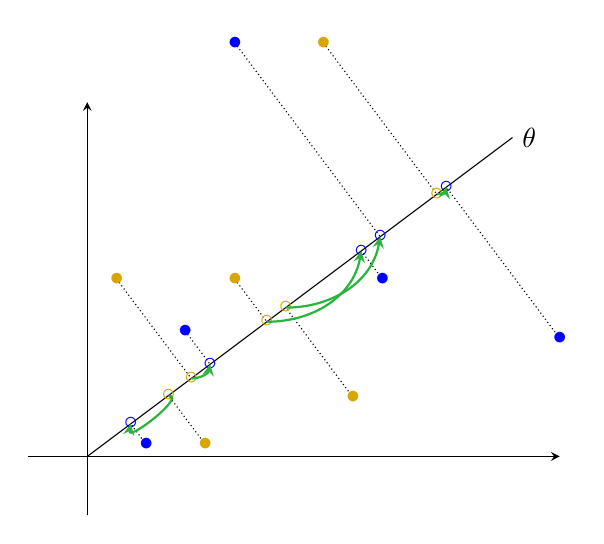
\begin{tikzpicture}
    \begin{scope}[xscale = 1.5, yscale = 1.5, >=stealth]
 \draw[->] (0, -.5) -- (0, 3) node [left] {}; %
      \draw[->] (-.5, 0) -- (4, 0) node [above] {} ; %
 \draw[-] (0, 0) -- (3.6, 2.7) node [right] {$\theta$} ; %
\draw[densely dotted] (.25, 1.5) -- (.88,.66 ) node [right] {} ;
\draw[darkyellow] (.88,.66) node {$\circ$} ;
\draw[darkyellow] (.25,1.5) node {$\bullet$} ;
\draw[densely dotted] (1, .1) -- (.688,.516 ) node [right] {} ;
\draw[darkyellow] (.688,.516 ) node {$\circ$} ;
\draw[darkyellow] (1,.1) node {$\bullet$} ;
\draw[densely dotted] (1.25, 1.5) -- (1.52,1.14 ) node [right] {} ;
\draw[darkyellow] (1.52,1.14 ) node {$\circ$} ;
\draw[darkyellow] (1.25,1.5) node {$\bullet$} ;
\draw[densely dotted] (2,3.5 ) -- (2.96,2.22) node [right] {} ;
\draw[darkyellow] (2.96,2.22 ) node {$\circ$} ;
\draw[darkyellow] (2,3.5) node {$\bullet$} ;
\draw[densely dotted] (2.25,.5) -- (1.68,1.26 ) node [right] {} ;
\draw[darkyellow] (1.68, 1.26) node {$\circ$} ;
\draw[darkyellow] (2.25,.5) node {$\bullet$} ;
\draw[densely dotted] (4, 1) -- (3.04,2.28) node [right] {} ;
\draw[blue] (3.04,2.28) node {$\circ$} ;
\draw[blue] (4,1) node {$\bullet$} ;
\draw[densely dotted] (.5, .1) -- (.368,.276) node [right] {} ;
\draw[blue] (.368,.276) node {$\circ$} ;
\draw[blue] (.5,.1) node {$\bullet$} ;
\draw[densely dotted] (1.25, 3.5) -- (2.48,1.86 ) node [right] {} ;
\draw[blue] (2.48,1.86) node {$\circ$} ;
\draw[blue] (1.25,3.5) node {$\bullet$} ;
\draw[densely dotted] (2.5,1.5) -- (2.32,1.74) node [right] {} ;
\draw[blue] (2.32,1.74) node {$\circ$} ;
\draw[blue] (2.5,1.5) node {$\bullet$} ;
\draw[densely dotted] (0.83, 1.06) -- (1.04,0.78) node [right] {} ;
\draw[blue] ( 1.04,0.78) node {$\circ$} ;
\draw[blue] (0.83, 1.06) node {$\bullet$} ;

\draw[->, thick, color=customgreen] (.88,.66) to[out=0, in=260] (1.04,0.78); % first pair
\draw[->, thick, color=customgreen] (.688,.516) to[out=0, in=260] (.368,.276); % second pair
\draw[->, thick, color=customgreen] (1.52,1.14) to[out=0, in=260] (2.32,1.74); % third pair
\draw[->, thick, color=customgreen] (1.68,1.26) to[out=0, in=260] (2.48,1.86); % fourth pair
\draw[->, thick, color=customgreen] (2.96,2.22) to[out=0, in=260] (3.04,2.28); % fifth pair
 \end{scope}
  \end{tikzpicture}
\caption{On the left, {we can see} the two discrete distributions $\mu$ 
{(blue points)} and $\nu$ {(yellow points)}. On the right, 
{we have} their projections $\pmu$ {(blue circles)} and $\pnu$ 
{(yellow circles)}
along the direction $\theta$. One then takes the increasing ordering of $\pmu$ 
and $\pnu$, 
{to obtain}
% obtains
the corresponding matchings {(green arrows)} and computes the cost 
% as in 
{following}
\autoref{eq:transport_ligne_2D_disc}.}
\label{fig:projection}
\end{center}
\end{subfigure}
\newline
\begin{subfigure}{\textwidth}
\begin{center}
\includegraphics[scale=0.335]{ReminderSW/Illust1DW.png}
\includegraphics[scale=0.3615]{ReminderSW/1DPlot1DW.png}
\caption{On the left, we have a plot of $\theta \mapsto \W(\pit \# \mu, \pit \# 
\nu)$ in polar coordinates, 
with 
{the distributions}
$\mu$ and $\nu$ 
% in \autoref{fig:projection}. 
{from \autoref{fig:projection} (top).}
The grey lines represent the 
angles where $\theta \mapsto \W(\pit \# \mu, \pit \# \nu)$ is not 
differentiable, the magenta line is the line of angle $\theta = \frac{\pi}{3}$ 
and the blue dot is a specific value of $\W(\pit \# \mu, \pit \# \nu)$ with the 
same angle. On the right, we have a $1D$ plot of $\theta \mapsto \W(\pit \# \mu, 
\pit \# \nu)$, here the hashed area represents $\SW(\mu,\nu)$ and again the 
vertical grey lines represent the values where $\theta \mapsto \W(\pit \# \mu, 
\pit \# \nu)$ is not differentiable. }
\label{fig:SW}
\end{center}
\end{subfigure}
\label{fig:proj&SW}
\caption{On the first row, \autoref{fig:projection} illustrates the 
% principle 
{computation}
of $\W(\pit \# \mu, \pit \# \nu)$ for a fixed $\theta$. On the second 
row, \autoref{fig:SW} gives a geometrical illustration of $\SW(\mu,\nu)$ with 
$\mu,\nu$ taken as in \autoref{fig:projection}.}
\label{fig:overallSWcomputation}
\end{figure}

% is easy in practice: the optimal transport
% solution is given by the monotone rearrangement of $\mu$ onto $\nu$.  
% This rearrangement maintains the ordering of points on the line. For
% discrete measures of $N$ points, it can be obtained in $O(N\log(N))$
% operations.  Writing $F_1$ and $F_2$ the cumulative distribution
% functions of $\rho_1$ and $\rho_2 $,

As a consequence, the Sliced Wasserstein distance between two discrete
probability measures $\mu =
\frac{1}{N}\sum\limits_{k=1}^N \delta_{x_k}$ and  $\nu =
\frac{1}{N}\sum\limits_{k=1}^N \delta_{y_k}$ on $\Rd$ (i.e. with
$(x_k)_{k=1,\hdots,N},(y_k)_{k=1,\hdots,N} \in \Rd$) can be rewritten{:} 
\begin{equation} \label{eq:SW_discrete}
\SW(\mu,\nu)= \frac{1}{N}\sum\limits_{k=1}^N\displaystyle\int_{\Sd}
(\langle x_{\sigma_{\theta}(k)} - y_{\tau_{\theta}(k)},\theta\rangle)^2
d\sd(\theta) = \frac{1}{N}\sum\limits_{k=1}^N\displaystyle\int_{\Sd}
(\langle x_{k} - y_{\tau_{\theta} \circ \sigma_{\theta}^{-1}(k)},\theta\rangle)^2
d\sd(\theta)  ,
\end{equation}
where
$\sigma_{\theta}$ and $\tau_{\theta}$ denotes respectively 
permutations which order the one dimensional  point sets $(\langle x_k,\theta\rangle)_{k=1,\hdots,N}$
and $(\langle y_k,\theta\rangle)_{k=1,\hdots,N}$. 
% \autoref{fig:projection}
{\autoref{fig:overallSWcomputation}}
illustrates the
computation of $\W(\pmu, \pnu)$ for two discrete measures in two dimensions 
{(\autoref{fig:projection})}, and 
% show
{shows}
how this quantity varies when $\theta$ spans $[0,2\pi]$ 
{(\autoref{fig:SW})}.

\noindent Since the permutations $\sigma_{\theta}$ and $\tau_{\theta}$
depends on the direction $\theta$, 
the 
{integrals}
in \autoref{eq:SW} and \autoref{eq:SW_discrete}
do not have closed forms. For this reason, practitioners rely on Monte
Carlo approximations of the form{:}
\begin{equation}
  \label{eq:SW_MC}
 \frac{1}{NM}\sum\limits_{k=1}^N \sum\limits_{j=1}^M\displaystyle
(\langle x_{\sigma_{\theta_j}(k)} - y_{\tau_{\theta_j}(k)},\theta_j\rangle)^2,
\end{equation}
where $\theta_1,\dots,\theta_M$ are i.i.d. and follow a uniform
distribution on the sphere.
 Classically, the convergence rate of such Monte Carlo estimations to
 SW is  $\mathcal{O}(\frac 1 {\sqrt{M}})$ ~{\citep{hammersley1964monte}}.
 In this context, it is natural to question the optimality of sampling
 methods to approximate SW efficiently in different scenarios.

\subsection{Regularity results on $\theta \mapsto \W(\pit \# \mu, \pit \# \nu)$} \label{sec:regularityProp}
The efficiency of sampling strategies used in numerical integration is
highly dependent on the regularity of the functions to be
integrated. For this reason, in the following we give some properties
of the function {(\autoref{fig:SW}):}
\begin{equation}
f: \theta\mapsto \W(\pit \# \mu, \pit \# \nu)\label{eq:f}
\end{equation}
on the
hypersphere $\Sd$. 
{We  first look at classical regularity properties of $f$}.

\begin{Prop}
{$f$ is Lipschitz on $\Sd$. 
}
\end{Prop}
\begin{proof}
{
Let $\mu$ and $\nu$ be two probability measures  with finite moments of order 2, and $\theta_1,\theta_2\in\Sd$. The triangular inequality on $W_2$ yields
$$\left| W_2(\pi_{\theta_1}\# \mu, \pi_{\theta_1}\# \nu) - W_2(\pi_{\theta_2}\# \mu, \pi_{\theta_2}\# \nu)\right| \leq W_2(\pi_{\theta_1}\# \mu,\pi_{\theta_2}\# \mu) +  W_2(\pi_{\theta_1}\# \nu,\pi_{\theta_2}\# \nu).$$
We also have
\begin{equation*}
W_2^2(\pi_{\theta_1}\# \mu,\pi_{\theta_2}\# \mu)  =  {\inf_{X\sim\mu, Y\sim\mu}\mathbb{E}\left[| \langle \theta_1 , X \rangle - \langle \theta_2, Y \rangle |^2\right]}
 \leq {\inf_{X\sim\mu}\mathbb{E}\left[|\langle \theta_1 - \theta_2, X\rangle |^2\right]}\\
 \leq \|\theta_1 - \theta_2\|^2 {\mathbb{E}_{X\sim\mu}[\|X\|^2]}.
\end{equation*}
We can show similarly that $W_2^2(\pi_{\theta_1}\# \nu,\pi_{\theta_2}\# \nu)\leq \|\theta_1 - \theta_2\|^2 {\mathbb{E}_{X\sim\nu}[\|X\|^2]}$. Thus 
$$\left| W_2(\pi_{\theta_1}\# \mu, \pi_{\theta_1}\# \nu) - W_2(\pi_{\theta_2}\# \mu, \pi_{\theta_2}\# \nu)\right| \leq \|\theta_1 - \theta_2\| \left( \sqrt{\mathbb{E}_{X\sim\mu}[\|X\|^2]}+\sqrt{\mathbb{E}_{X\sim\nu}[\|X\|^2]}\right).$$}
\end{proof}
{Since $f$ is Lipschitz continuous, it is  differentiable almost everywhere.
However the previous result does not give us the set where $f$ is non differentiable. In the following we give a more complete proof when $\mu$ and $\nu$ are discrete following the notations introduced in \autoref{sec:def}.}

\begin{Prop}
When $\mu$ and $\nu$ are finite discrete measures, $f$ piecewise $\mathcal{C}^{\infty}$
($\mathcal{C}_{pw}^{\infty}$) and Lipschitz on $\Sd$. 
 \end{Prop}
\begin{proof}
For discrete measures  $\mu =
\frac{1}{N}\sum\limits_{k=1}^N \delta_{x_k}$ and  $\nu =
\frac{1}{N}\sum\limits_{k=1}^N \delta_{y_k}$ on $\Rd$, $f$ can be
  rewritten as 
  \begin{equation}
f(\theta) = \min_{\sigma \in \Sigma_N} f_{\sigma}(\theta), \text{
    where } f_{\sigma}(\theta) = \sum_{k=1}^N \langle
  x_k-y_{\sigma(k)} | \theta \rangle ^2,\label{eq:f_as_min}
\end{equation}
where $\Sigma_N$ is the set of permutations of $\llbracket 1,N\rrbracket$.
We assume that the $\{x_i\}$ (resp. $\{y_j\}$) are all distinct. 
In the following, we study the regularity of $f$ as a function of
$\R^d$ and deduce the regularity properties of its restriction
$f_{|\Sd}$. 
Observe that each $f_{\sigma}$ defines a quadratic function on $\R^d$
and $f$, as a
minimum of a finite number of such functions, is continuous 
and also piecewise  $\mathcal{C}^{\infty}$ on $\R^d$. Since $f$ is
continuous on $\R^d$, its restriction to $\Sd$ is also continuous. To show that this restriction to $\Sd$ is also in
$\mathcal{C}_{pw}^{\infty}$, it is enough to observe that the set of
points of $\R^d$ where $f$ is not differentiable is included in the
finite union of hyperplanes
$\left(\cup_{i,j} \tspan(x_i - x_j)^{\perp} \right)\bigcup \left(\cup_{k,l}\tspan(y_k -
y_l)^{\perp}\right)$, since these {hyperplanes} are the locations where the
minimum in~\autoref{eq:f_as_min} jumps from a permutation $\sigma$ to
another one (see \autoref{fig:hyperplanes} as an illustration of those hyperplanes). Each of these
hyperplanes intersect $\Sd$ on a great circle, and we call $\mathcal{U}$ 
the sphere minus this finite union of great circles. The open set
$\mathcal{U}$ (which is dense in $\Sd$) can be written as the union $\bigcup_{k=1}^p V_k$ of a finite number of
connected open sets $V_l$, such that on each $V_l$, the permutation
$\sigma$ which attains the minimum in~\autoref{eq:f_as_min}  is
constant and unambiguous. We write this permutation $\sigma_l$. On
each $V_l$, $f_{|\Sd} = {f_{\sigma_l}}$, thus is  
$\mathcal{C}^{\infty}$ on $V_l$ and its derivative can be
obtained as the projection of  $\nabla f_{\sigma_l}$ on the
hypersphere. For $\theta \in \mathcal{U}$, writing $\sigma_{\theta}$
the permutation which attains the minimum in~\autoref{eq:f_as_min}  for
the direction
$\theta$, this derivative can be written
{\begin{equation}
  \nabla_{(d-1)} f (\theta) = 2 \left( \sum_{k = 1}^{N} \left( \langle x_{k} -
  y_{\sigma_\theta(k)} | \theta \rangle(x_{k} - y_{\sigma_\theta(k)} ) 
  -     \langle x_{k} -
  y_{\sigma_\theta(k)} | \theta \rangle ^2 \theta\right)\right).
  \label{eq:fderivative}
\end{equation}}
Since these derivatives are upper bounded on the compact set $\Sd$, it
follows that $f$ is also Lipschitz on  $\Sd$.\\
In the case where several $x_i$ (or $y_j$)  are equal,
several of the functions $f_\sigma$ coincide.  For instance, if $x_1 =
x_2$, the values of $\sigma(1)$ and $\sigma(2)$ can be exchanged
without modifying $f_\sigma$. By eliminating all the redundant
functions, we can make the same reasoning as before to show the same
regularity results on $f$.  In this case, all the pairs $(x_i,x_j)$
with $x_i = x_j$ should be
removed when constructing the set of great circles dividing the hypersphere.
\end{proof}


\begin{figure}[!h]
\begin{center}
\includegraphics[scale=0.45]{ReminderSW/hyperplanesNew3.png}
\caption{Illustration of the open subsets $\bigcup_{k=1}^p V_k$ and their intersection with the hyperplanes  $\left(\cup_{i,j} \tspan(x_i - x_j)^{\perp} \right)\bigcup \left(\cup_{k,l}\tspan(y_k -
y_l)^{\perp}\right)$, in the specific case of two measures made of two diracs 
{$\mu = \displaystyle\frac{1}{2} \sum\limits_{i = 1}^2 \delta_{x_i}$ with $ 
x_1,x_2 = (1,0,0)^T, (0,-1,0)^T$ and $\nu = 
\displaystyle\frac{1}{2}\sum\limits_{i = 1}^2 \delta_{y_i} $ with $y_1,y_2 = 
(0,0,1)^T,(0,0,-1)^T$}. The hyperplanes divide the sphere into the colored 
sections where $\sigtheta$ and $\tautheta$ are constant. 
}
\label{fig:hyperplanes}
\end{center}
\end{figure}

\noindent The following proposition will also be useful in the next sections.
\begin{Prop} \label{prop:Sobol}
  $f \in H^{1}(\Sd)$, where, for $\alpha\in\N$, the Sobolev space $H^{\alpha}(\Sd)$ is defined as~\citep{Hebey1996} 
  \[H^{\alpha}(\Sd) = \{ h\in L^2(\Sd)\ |\ \partial^{|j|}h\in L^2(\Sd), 0 \leq |j| \leq \alpha\},\]
with $j$ a multi-index and $\partial^{|j|}$ the partial mixed derivative of order $|j|$ on $\Sd$.
  \end{Prop}
  \begin{proof}
  We have seen previously that $f$ is continuous and piecewise $\mathcal{C}^{\infty}$, piecewise quadratic to be more precise. Thus its weak derivative is piecewise linear with discontinuities on a finite union of hyperplanes, which is $L^2$.
  \end{proof}




\section{Reminders on sampling strategies on the sphere and their theoretical guarantees}\label{sec:Sampling}
{In this section, we present the different 
sampling methods for numerical integration on $\Sd$ considered in this paper, 
before comparing them experimentally in \autoref{sec:Exp}. This paper addresses 
three main types of sampling: random sampling, discrepancy-based sampling, and a 
control variate approach. The first type includes the classical Monte Carlo 
(M.C.) method (\citep{hammersley1964monte}, \citep{lemieux2009monte}) on the 
sphere and its variant called orthonormal sampling 
\citep{rowland2019orthogonal}. The second one relies on a concept called the 
discrepancy (\citep{lemieux2009monte},\citep{dick2010digital}) of a point set, 
which represents the number of points in a unit of volume, and can be divided 
into two categories: low-discrepancy sequences (or digital nets) and point sets 
(or lattices). {Among the former category, we also investigate a method based on a spherical sliced-Wasserstein type discrepancy~\citep{bonet2023sphericalslicedwasserstein}.} The last type details a control variates method 
~\citep{lemieux2009monte} using spherical harmonics ~\citep{Muller1998} for this 
purpose ~\citep{leluc2024slicedwassersteinestimationsphericalharmonics}. We will 
also determine which method, and under which conditions, is theoretically 
suitable based on the regularity properties established in 
\autoref{sec:regularityProp}. \autoref{tab:summarySamplingMethods} presents a 
taxonomy of all the sampling methods explored in this paper. It details which 
method's convergence rate result is \textbf{independent from the dimension} 
({i.e.} the dimension does not appear in the asymptotic rate), which one 
can be \textbf{computed independently} 
({i.e.} each sample can be generated 
independently from the others), and which one can be \textbf{computed and 
stored} in advance.} 

\begin{table}[h!]
\resizebox{\linewidth}{!}{
\begin{tabular}{|c|c|c|c|c|}
\hline
Sampling types &  
{Dimension independence}
& Independent computation & 
{Possible pre-computation}
\\
\hline
\textbf{Random Sampling} &  &   & \\
\hline
Uniform Sampling & x & x & x  \\
Orthonormal Sampling & x & x  & x \\
\hline
\textbf{Based on discrepancy} & & & \\
\hline
Riesz Point Set / Riesz Point Set Randomized &  &  & x \\
Fibonacci Point Set / Fibonacci Point Set Randomized &  &  & x \\
Sobol / Sobol Randomized mapped on $\Sd$ &  & x & x \\
Halton / Halton Randomized on $\Sd $ &  & x & x \\
{Spherical Sliced Wasserstein Discrepancy} & {x} & & {x}\\ 
\hline
\textbf{Control variates} & & & \\
\hline
Spherical Harmonics Control Variates &  &  & \\
\hline
\end{tabular}}
\caption{{Taxonomy of the three types of sampling methods 
{investigated in this paper.}
}}
\label{tab:summarySamplingMethods}
\end{table}

{\autoref{tab:summaryConvergenceAndComplexity}  
gives a summary of the convergence rate and computational complexity of each sampling method explored in this paper. In this table $n_M = o\bigg(M^{1/\big(2(d-1)\big)}\bigg)$.}

{
\begin{table}[h!]
\resizebox{\linewidth}{!}{
\begin{tabular}{|c|c|c|c|c|}
\hline
{Sampling types} & 
{Theoretical convergence rate}
& {Time complexity} & {Space complexity}
\\
\hline
{\textbf{Random Sampling}} &  &  & \\
\hline
{Uniform Sampling} & {$\mathcal{O}(1/\sqrt{M})$} & {$\mathcal{O}(M)$}& {$\mathcal{O}(M)$}\\
{Orthonormal Sampling} & {None} & {$\mathcal{O}(M)$}& {$\mathcal{O}(M)$}\\
\hline
{\textbf{Based on discrepancy}} & & &\\
\hline
{Riesz Point Set / Riesz Point Set Randomized} & {$1/M$ on $\mathbb{S}^1$, Not applicable otherwise}  & {$\mathcal{O}(M^2)$} & {$\mathcal{O}(M)$} \\
{Fibonacci Point Set / Fibonacci Point Set Randomized} & {Not applicable} &  {$\mathcal{O}(M)$} & {$\mathcal{O}(M)$}\\
{Sobol / Sobol Randomized mapped on $\Sd$} & {None} & {$\mathcal{O}\big(M \text{log}_b^2(M)\big)$} & {$\mathcal{O}(M)$} \\
{Halton / Halton Randomized on $\Sd $} & {None} & {$\mathcal{O}\big(M \text{log}_b^2(M)\big)$} & {$\mathcal{O}(M)$}\\
{Spherical Sliced Wasserstein Discrepancy} & {None} & {$\mathcal{O}(M\text{log}(M))$} & {$\mathcal{O}(M)$}\\
\hline
{\textbf{Control variates}} & & &\\
\hline
{Spherical Harmonics Control Variates} & {$\mathcal{O}\big(1/(n_M \sqrt{M})\big)$} & {$\mathcal{O}(M)$} & {$\mathcal{O}(M)$}\\
\hline
\end{tabular}}
\caption{{Convergence rate, time complexity and spacial complexity (w.r.t the sampling number) summary of the sampling methods 
studied in this paper.
}}
\label{tab:summaryConvergenceAndComplexity}
\end{table}
}

\subsection{Random samplings} \label{sec:Rand}

{We first explore} classical strategies for randomly generating points on the sphere: uniform sampling \citep{hammersley1964monte} and orthonormal sampling \citep{rowland2019orthogonal}. These strategies are the most commonly used for estimating $\SW$, and their convergence rates do not depend on the dimension of the input measures.


\subsubsection{Classical Monte Carlo} \label{sec:unif}

{The classical Monte Carlo method uses uniform random sampling to generate the projection angles. 
For $(\theta_M)_{M\in\mathbb{N}^*}$ i.i.d. samples of $\sd$~\footnote{In practice, to simulate a random variable $\theta\sim\sd$, one takes a normal random variable $Z\sim\mathcal{N}(0, I_d)\neq 0$ and chooses $\theta = \frac{Z}{\| Z \|} \sim \sd$ \citep{asmussen2007stochastic}.}, we write the Monte Carlo Estimator 
\begin{equation}
    X_M :=\displaystyle\frac{1}{M}\sum\limits_{i = 1}^{M} f(\theta_i) \text{ with } M\in\mathbb{N}^* . 
    \label{eq:mcestimator}
\end{equation}
The law of large numbers ensures that $X_M$ converges a.s. to $\SW(\mu,\nu) = \mathbb{E}_{\theta \sim \sd}[f(\theta)]$ as $M$ goes to infinity. Moreover, the rate of convergence for this unbiased estimator  is given by 
\begin{equation}\label{eq:convUnif}
    \sqrt{\mathbb{V}[X_M]} = \sqrt{\frac {\mathbb{V}[X_1]}{M}} = \frac {{\sigma}}{\sqrt{M}},
    \end{equation}
where $\sigma^2 = \mathbb{V}[f(\theta)] = \displaystyle\int_{\Sd} f^2(\theta) ds_{d-1}(\theta) - \SWsq(\mu,\nu) < +\infty$.
{This convergence rate in \autoref{eq:convUnif} does not depend on the dimension of the input measures}. 
In order to derive confidence intervals for $\SW(\mu,\nu)$, we can rely on the Central Limit Theorem~\citep{fischer2010history} , which states that 
\begin{equation*}\label{eq:CLTSW}
    \sqrt{M}\frac{[X_M - \SW(\mu,\nu)]}{\mathbb{\sigma}} \xrightarrow[M\rightarrow +\infty]{\mathcal{L}} \mathcal{N}(0,1),
\end{equation*}
This allows us to compute confidence intervals for $\SW(\mu,\nu)$ by using the quantiles of the standard normal distribution.}
\noindent {This means that} for $M$ large enough,  $\mathbb{P}\left(X_M - \SW(\mu,\nu) \in \left[  -\frac{\sigma q_{1 - \alpha/2}}{\sqrt{M}} , \frac{\sigma q_{1 - \alpha/2}}{\sqrt{M}}\right]\right) {\xrightarrow[M\rightarrow +\infty]{}} 1 - \alpha$, with $\alpha$ in $[0,1]$  and $q_{1 - \alpha/2}$ the quantile {of level $1 - \alpha /2$} of $\mathcal{N}(0,1)$. 
One strategy for choosing $M$ is taking $M$ such that $\frac{\sigma q_{1 - \alpha/2}}{\sqrt{M}} \leq \varepsilon$ with $\varepsilon\geq 0$ a chosen {precision}.  The value of $\sigma$ being unknown, a possibility is to plug a consistent  estimator of $\sigma^2$, such as
$$\hat{\std}_M^2 = \frac{1}{M}\left[\displaystyle\sum\limits_{i = 1}^M f(\theta_i)^2 - X_M^2\right].$$
\citet{xu2022central} provide an alternative criteria for choosing $M$, however it is quite impractical as it {requires} to compute the Wasserstein distance between $\mu$ and $\nu$.


\subsubsection{Orthonormal sampling} \label{ortho}

{A variant of the uniform sampling covered in \autoref{sec:unif} was introduced by \citep{rowland2019orthogonal}, which presents a simple variant for the previous Monte Carlo estimator $X_M$ by sampling random orthonormal bases. This method is inspired by variance reduction techniques known as stratification \citep{lemieux2009monte}.
Let $O(d)$ be the orthogonal group in $\R^d$. For $(\Theta_P)_{P\in \N^*} \sim \mathcal{U}\big(O(d)\big)$, denoting $\theta_1,\hdots,\theta_M$ all the columns of the matrices $\Theta_1,\hdots,\Theta_K$, we define $Y_M =\displaystyle\frac{1}{M}\sum\limits_{i = 1}^{M} f(\theta_i)$. It is easy to show that each $\theta_i$ follows the uniform distribution on $\Sd$~\citep{rowland2019orthogonal}. As a consequence, the estimator $Y_M$ is still unbiased. Although it is not possible to show that $Y_M$ has a smaller variance than $X_M$ in general, this estimator is most of the time more efficient than $X_M$ in our experiments and show an equivalent or better rate of convergence in practice. This might be due to the fact that the diversity of the samples is increased by the orthonormality constraint.}

\begin{Rk}
 Other fully random point processes on $[0,1]^2$ or $\mathbb{S}^2$ suitable for Monte Carlo integration are studied in the literature. Among them, we can mention Determinantal Point Process (DPP). Recent works, such as \citep{feng2023determinantalpointprocessesspheres}, have proposed DPP methods directly on the sphere $\mathbb{S}^2$. Unfortunately, due to the lack of publicly available implementations, we could not experiment efficiently with these methods.
\end{Rk}


\subsection{Sampling strategies based on discrepancy}

We examine in this section two different types of deterministic sampling based on discrepancy: low-discrepancy sequences (digital nets) and low-discrepancy point sets (lattices). They were developed to replace random sampling, expecting to have a better convergence rate than the classical Monte Carlo method. 

\subsubsection{Low-discrepancy sequences} \label{sub:lds}

Quasi-random sequences, better known as low-discrepancy sequences (L.D.S.), are 
sequences mimicking the behavior of random sequences while being entirely 
deterministic. {To date, these sequences are only defined on the unit 
{hypercube}
$[0,1]^d$. We introduce below a first definition of discrepancy 
(\citep{lemieux2009monte},\citep{dick2010digital})}.
\begin{D}
The discrepancy of a set of points $P = \{u_1, \hdots, u_M\}$ in {$[0,1]^d$} is defined as
$$D_M(P) = \sup_{I\in \mathcal{I}} \Bigg| \frac{| P \cap I |}{M} - \lambdim(I)\Bigg|,$$
where  $|A|$ denotes the cardinal of a set $A$, $\lambdim$ is the $d$-dimensional Lebesgue measure and
 $\mathcal{I} = \{\prod\limits_{i = 1}^d [a_i,b_i[\ |\ 0 \leq a_i < b_i \leq 1\}$. The star-discrepancy $D_M^*(P)$ is defined the same way with $\mathcal{I}^{*} = \{\prod\limits_{i = 1}^d [0,b_i[ \ |\ 0 \leq  b_i \leq 1\}$.
\end{D}

We can now provide a definition of a Low discrepancy sequence (L.D.S.).
\begin{D}
{Let $(u_m)_{m\in\N^*}$ be a sequence in $[0,1]^d$. Denoting $P_M = \{u_1, \hdots, u_M\}$ for any $M\in\N^*$, $u$ is a L.D.S. if
$$D_M^*(P_M) \xrightarrow[M \to +\infty]{} 0.$$}
\end{D}




{The notion of discrepancy is important because it is related to the error made when approximating an integral on the hypercube by its Monte Carlo approximation.} {This relation is made explicit by the Koksma-Hlawka inequality (\citep{lemieux2009monte}; \citep{dick2010digital}; \citep{brandolini2013koksma}).}

This inequality requires to introduce the notion of Hardy-Krause variation $V_h$ of a function $h$ on $[0,1]^d$ \citep{aistleitner2016functions}, which is out of the scope of this paper, but can be broadly understood as a measure of the oscillation of $h$ on the unit cube $[0,1]^d$.
\begin{Prop}[Koksma-Hlawka inequality]
Let {$h:[0,1]^d \rightarrow \mathbb{R}$} have bounded variation $V_h$ on {$[0,1]^d$} in the sense of Hardy-Krause \citep{aistleitner2016functions}. Then for $\{u_1,\hdots,u_M\}$ a point set in {$[0,1]^d$}, we have
\begin{equation}\label{eq:KHIneq}
\Bigg |\frac{1}{M}\displaystyle\sum\limits_{k=1}^M h(u_k) - \displaystyle\int_{S} h(x)d\lambdim(x) \Bigg | \leq V_h D_M^*(u_1,\hdots,u_M).
\end{equation}
\end{Prop}
\noindent The proof of this inequality and basic results on discrepancy theory can be found in\citep{kuipers2012uniform} and \citep{dick2010digital}. \autoref{eq:KHIneq} shows that the absolute error made {by the Monte Carlo approximation} is {upper} bounded {by a term depending only on $h$} and the star discrepancy. Compared to the Central Limit Theoreom, this inequality is not probabilistic and not asymptotic, the bound being valid for every $M \in \mathbb{N}^*$.  An important limitation is the term $V_h$, which is impractical to compute directly. When $d = 1$, this term is exactly the total variation of $h$, but in general, it is only {upper} bounded by the total variation. 
In the case of our function $f$ involved in the estimation of $SW$, $V_f < +\infty$ holds since $f$  is Lipschitz continuous. Another limitation of the previous bound is that the rate of convergence of the star discrepancy $D_M^*$ of a sequence is most of the time not explicit and difficult to compute~\citep{owen2005multidimensional}. 

Nevertheless, this proposition ensures that if the rate of convergence of the star discrepancy of a sequence is better than $O(\frac 1 {\sqrt{M}})$, for $M$ large enough the approximation of the quasi Monte Carlo approximation using this sequence will outperform the one of classical Monte Carlo. 

{In the following, we present two L.D.S. defined on the unit square $[0,1]^d$, and see how their star discrepancy decreases with $M$. We then focus on practical methods to map these sequences from the hypercube to the hypersphere $\Sd$.}

\paragraph{Halton sequence} \label{par:Halton}\mbox{} \\

The Halton sequence $(u_i)_{i\in\N} \in (\Rd)^{\N}$ \citep{halton1964algorithm} is a generalization of the von der Corput sequence \citep{vdc1935}. In the following, we write, for any integer $i$, $c_l(i)$ the coefficients from the expansion of $i$ in base $b$, and we define the radical-inverse function in base $b$ as 
$$
\phi_b(i) = \displaystyle\sum\limits_{l = 0}^{+\infty} c_l(i)b^{{-}l-1},\forall i \in \mathbb{N}.
$$ 
The Halton sequence in dimension $d$ is then defined as
$$
u_i = (\phi_{b_1}(i),\hdots,\phi_{b_d}(i))^T,
$$
where $b_i$ is chosen as the i-th prime number.

\paragraph{Sobol sequence} \label{par:Sobol}\mbox{} \\

This sequence uses the base $b = 2$. To generate the $j$-th coordinate of the $i$-th point $u_i$ in a Sobol sequence \citep{sobol1967distribution}, one needs a primitive polynomial of degree $n_j$ in $\Zq[X]$,
$$
X^{n_j} + a_{1,j}X^{n_j - 1} + a_{2,j}X^{n_j - 2} + \hdots + a_{n_j-1,j}X + 1.
$$
{This polynomial is used to define} a sequence of positive integers $(m_{k,j})$ by recurrence, with $+_{\Zq}$ the inner law of $\Zq$:
$$
m_{k,j} = 2a_{1,j}m_{k-1,j}+_{\Zq} 2^2a_{2,j}m_{k-2,j} +_{\Zq} \hdots +_{\Zq} 2^{n_j}m_{k-n_j,j} +_{\Zq} m_{k-n_j,j}.
$$
The values $m_{k,j}$, {for $1\leq k \leq n_j$,} can be chosen chosen arbitrarily provided that each is odd and less than $2^k$. Then one {generates} what is called direction numbers:
$$v_{k,j} = \frac{m_{k,j}}{2^k}.$$
The $j$-th coordinate of $u_i$ is then obtained as
$$
u_{i,j} = \displaystyle\sum\limits_{k = 1}^{+\infty} c_k(i) v_{k,j}.
$$

\paragraph{Convergence rate of Halton and Sobol sequences} \label{par:convHaltonSobol}

Both sequences (Halton and Sobol) have a star discrepancy which converges to $0$ (which means that they are indeed L.D.S.). The convergence rate is given by the following property~\citep{niederreiter1988low}~\citep{owen2019monte}.
\begin{Prop}
Let $(u_m)_{m\in\mathbb{N}^*}$ be either the Halton sequence or Sobol sequence in $[0,1]^d$. Then for $M\geq 1$, we have
$$D_M^{*}(u_1,\hdots,u_M)\leq c_d \frac{log(M)^d}{M}$$
where $c_d$ is a constant that depends only on the dimension.
\end{Prop}
Thanks to~\autoref{eq:KHIneq}, {for any function $h$ such that $V_h<+\infty$ (which is the case for our function $f$)}, this implies  a convergence rate of the Monte Carlo estimator using these sequences in $\mathcal{O}(\frac{log(M)^d}{M})$, which means $\mathcal{O}(M^{-1+\epsilon})$ for every $\epsilon >0$. This convergence rate  is better than the one of classical Monte Carlo with i.i.d. sequences, {even if the rate of convergence slows down when the dimension increases, because of the term $\log(M)^d$.} 
{
\begin{Rk}
Note that L.D.S. are designed to mimic the behavior of a random uniform sampling in $[0,1]^d$ while being completely deterministic. This deterministic behavior leads to patterns in the sampling; because of those patterns, the higher the dimension, the harder it is for those to fill the "gaps" in $[0,1]^d$.
Moreover, the term $\text{log}(M)^d$ implies that one needs $M$ to be very large (exponential) to get the same level of space coverage in high dimension than in low dimension.
\end{Rk}
}
{
\begin{Rk}
Observe that both for Sobol and Halton sequences, {generating $M$ values} has a complexity in $\mathcal{O}\big(M log_b^2(M)\big)$, where $b$ is the base (or smallest basis for Halton) chosen.
\end{Rk}
}

\paragraph{L.D.S. on the sphere} \label{par:ldsSphere}\mbox{} \\
\noindent To our knowledge, there is no true L.D.S. on the unit sphere $\Sd$ for $d \geq 3$, this question remaining an active research area. Practitioners typically map L.D.S. from the hypercube to the hypersphere, using one of the methods described below: 
\begin{itemize}\label{item:Methods}
\item[$\bullet$] \textbf{Equal area mapping} ~\citep{Aistleitner2012}: this method is only defined for mapping points in the unit square to $\mathbb{S}^2$. Denoting $(z_1,z_2)\in [0,1[^2$,  one gets a point $u = \Phi(2\pi z_1, 1-2z_2)$ on $\mathbb{S}^2$ with:
\begin{equation}\label{eq:EqArea}
\Phi(\eta, \beta) = \left( \sqrt{1 - \beta^2}\tcos(\eta), \sqrt{1 - \beta^2}\tsin(\eta), \beta\right),\ \eta,\beta\in[0,1[.
\end{equation}

\item[$\bullet$] \textbf{Spherical coordinates}~\citep{arfken2011mathematical}: This method maps the points from an L.D.S. in $[0,1]^{d-1}$ to $\Sd$ by using the spherical coordinates.  Unfortunately, we found that the resulting sampling is usually not competitive compared to other sampling methods.

\item[$\bullet$] \textbf{Normalization onto the sphere} ~\citep{basu2016}: {An L.D.S. is generated 
in the $d$-hypercube $[0,1]^d$ and mapped to $\R^d$ using the inverse cumulative 
distribution function of the standard normal distribution (separately on each 
dimension).  Then each point in the 
{resulting}
sequence is normalized by its norm to map it onto $\Sd$. }

\end{itemize}


\textbf{Specific case of $\mathbb{S}^2$.} \\
In the specific case of $\mathbb{S}^2$, it has been shown by~\citet{Aistleitner2012} that if $u$ is an L.D.S in $[0,1]^2$ and $\Phi$ the equal area mapping defined in \autoref{eq:EqArea}, the spherical cap discrepancy $D_{\mathbb{L}_2,M}\big(\Phi(P)\big)$ (see definition \autoref{eq:SphereCal} in the next section) of the mapped sequence is in $\mathcal{O}\left(\frac{1}{M^{1/2}}\right)$. However, their experiments showed that the correct order seems rather to be $\mathcal{O}\left(\frac{log^c (M)}{M^{3/4}}\right)$ for $1/2\leq c \leq 1$.


\subsubsection{Deterministic point sets on $\Sd$} \label{sec:QMCSphere}

This section details different methods to design well distributed point sets on $\Sd$. Contrary to the L.D.S. defined above,  these point sets are defined directly on the sphere, in order to be approximately uniformly distributed on $\Sd$. To measure this uniformity, we can rely on the notion of spherical cap on the sphere: a spherical cap of center $c\in\Sd$ and $t\in [-1,1]$ is defined as
\begin{equation}
C(c,t) = \{ x \in \Sd\ | \ \langle x , c \rangle > t\}.
\end{equation}\label{eq:sphereCap}

In other words, a spherical cap is the intersection of a portion of the sphere and a half-space (see \autoref{fig:sphericalcap} for an illustration). 
\begin{figure}[!h]
\begin{center}
\includegraphics[scale=0.25]{ReminderSampling/sphericalcapnew.png}
\caption{Illustration of a spherical cap on $\mathbb{S}^2$. The circle represents the intersection of the plane $\langle x, c \rangle = t$ with the sphere, and the purple colored area is the cap $C(c,t)$ as noted in \autoref{eq:sphereCap}.}
\label{fig:sphericalcap}
\end{center}
\end{figure}


To the best of our knowledge, there is no equivalent to the Koksma-Hlawka inequality for the sphere in full generality~\citep{brauchart2011optimal}. 
A sequence of points $\{u_n\}$ on $\Sd$ is said asymptotically uniformly distributed on $\Sd$ if for every spherical cap $C$, the proportion of points inside the cap, converges to the measure of the cap $\sd(C)$. It can be shown that this assumption is equivalent to assume that for every continuous function $h$, the Monte Carlo approximation $\frac 1 M \sum_{k=1}^M h(u_k)$ converges to $\mathbb{E}_{\theta \sim \sd}[h(\theta)]$. 

In order to get a non asymptotic notion of the uniformity of a point set on $\Sd$, we can rely on different notions of spherical cap discrepancy on the sphere, defined as follows.


\begin{D}
The spherical cap max-discrepancy of a point set $P_M$ of size $M$ is defined as~\citep{marzo2021discrepancy}:
\begin{equation*}
    D_{max}(P_M) = \sup_{c\in \Sd ,t \in [-1,1]}\left\lbrace  \bigg | \frac{|P_M \cap C(c,t)|}{M} - s_{d-1}\big(C(c,t)\big)\bigg| \right\rbrace.
\end{equation*}\label{eq:Spheremax}
The spherical cap $\mathbb{L}_2$-discrepancy of a point set $P_M$ of size $M$ is defined as~\citep{brauchart2011optimal}:
\begin{equation*}
D_{\mathbb{L}_2}^2(P_M) = \left\lbrace \int_{-1}^1 \int_{\Sd} \bigg | \frac{|P_M \cap C(c,t)|}{M} - s_{d-1}\big(C(c,t)\big)\bigg|^2 ds_{d-1}(c) dt\right\rbrace ,
\end{equation*}\label{eq:SphereCal}
where $C(c,t)$ is  a spherical cap of center $c$ and height $t$.
\end{D}
Again, the idea is to compare the proportion of points in $P_M$ that fall inside a spherical cap with the measure of the cap. This comparison is done for all possible caps on the sphere, and $D_{max}$ represents the worst error over all possible caps, while $D_{\mathbb{L}_2}^2$ represents the average squared error over all possible caps.


When using 
{Q.M.C.}
on the hypersphere to approximate the integral of functions $h$, 
another notion often used in the literature is the worst-case (integration) error (W.C.E.) on a Banach space of functions, which is the largest possible error made by the method on the space. 
For instance, on $H^{\alpha}(\Sd)$,
\begin{D}
For $P_M = \{ u_1,\hdots, u_M\}$, for $\alpha \in \N$
\begin{equation*}
WCE\Big(P_M,H^{\alpha}(\Sd)\Big)= \sup_{h\in H^{\alpha}(\Sd)} \bigg |\displaystyle \frac{1}{M} \sum\limits_{m=1}^M h(u_m) - \frac{1}{s_{d-1}(\Sd)}\int_{\Sd} h(w) ds_{d-1}(w) \bigg |.
\end{equation*}
\end{D}
\noindent Under some regularity condition, a sufficient and necessary one being $\alpha \geq \frac{1}{2} + \frac{d - 1}{2}$ for $H^{\alpha}(\Sd)$, \citet{Brauchart_2013} show that optimizing the spherical cap $\mathbb{L}_2$-discrepancy is equivalent to optimizing the W.C.E. thanks to the Stolarsky's invariant principle ~\citep{stolarsky1973}.
In the case of our function $f$, we have seen that $f$ is regular enough in the specific case of $\mathbb{S}^1$, since $f\in H^{\alpha} (\mathbb{S}^1)$ with $\alpha = 1 = \frac{1}{2} + \frac{1}{2}$. However in dimension larger than $3$, this result does not hold anymore since $f$ does not belong to any Sobolev space $H^{\alpha} (\mathbb{S}^d)$ with $\alpha > 1$.

\paragraph{Fibonacci point set on $\mathbb{S}^2$}\mbox{}\\
\noindent {Denoting $\varphi$ the polar angle and $\chi$ the azimuthal angle 
forming the geographical coordinates $(\varphi, \chi)$,  we retrieve the 
Cartesian coordinates $(x,y,z)$ using the spherical coordinates 
(see~\autoref{fig:sphericalcoord} for 
{an}
illustration).} Noting $\phi = \frac{1 + \sqrt{5}}{2}$ the golden 
ratio, {the $m$-th point $u_m = (\varphi_m, \chi_m)$ of the Fibonacci} {point} set is given by
\begin{align*}
\varphi_m &= \tacos\left(\frac{2m}{2M + 1}\right),\\
\chi_m &= 2m\pi \phi^{-2}.
\end{align*}
It is a simple and  efficient way, convergence rate wise, to generate points on $\mathbb{S}^2$ for the quasi-Monte Carlo method {but it} is only defined on $\mathbb{S}^2$. The complexity of the generation is linear in $M$, and according to \citep{Marques2013}, the corresponding convergence rate for the W.C.E. and the $\mathbb{L}_2$-spherical cap discrepancy is in $\mathcal{O}(\frac{1}{M^{3/4}})$. For an extensive list of other popular point configurations on $\mathbb{S}^2$, see \citep{hardin2016comparison}. 


\begin{figure}[!h]
\begin{center}
\includegraphics[scale=0.18]{ReminderSampling/sphereCoords2.png}
\caption{Illustration of the spherical coordinates in $\R^3$ for points on the sphere $\mathbb{S}^2$.}
\label{fig:sphericalcoord}
\end{center}
\end{figure}


\paragraph{Equi-distributed points generated by the discrete s-Riesz energy} \label{par:Riesz} \mbox{}\\

Another classical way to define equi-distributed point sets on the hypersphere is to rely on optimization. In such methods, the point set $P_M$ is defined as the minimizer of a certain energy functional $E_s$,
\begin{equation*}
    P^*_M := \argmin_{u_1,\hdots,u_M \in \Sd} E_s(u_1,\hdots, u_M).
\end{equation*}
The most common energy functional is the s-Riesz energy, which is defined as follows. 
\begin{D}
For $s \geq 0$ and $P_M = \{ u_1, \hdots, u_M\}$ a set of points on $\Sd$, the s-Riesz energy of $P$ is defined as
\begin{equation*}
E_s(P_M) = 
\begin{cases}
\displaystyle\sum\limits_{i\neq j} \frac{1}{\| u_i - u_j\|^s} & \text{if} \ s > 0,\\
\displaystyle\sum\limits_{i\neq j} \text{log} \frac{1}{\| u_i - u_j\|} & \text{if} \ s = 0.
\end{cases}
\end{equation*}
\end{D}

The resulting point set is called a minimal $s$-energy configuration. {The s-Riesz energy can also be defined for $s < 0$, in this case the point set $P_M$ is obtained as the maximizer of $E_s= \displaystyle\sum\limits_{i\neq j} \| u_i - u_j\|^s$~\citep{brauchart2011optimal}.} Minimising $E_s$  is non trivial, the functional being not convex, and the problem becomes more complex when the dimension increases. 
Minimal energy configuration points for $E_s$ are called Fekete points and it is known that for $0\leq s < d$, these sets are asymptotically uniformly distributed with respect to the normalized surface measure $s_{d-1}$, which means that Monte Carlo estimates using the Fekete points converge to the integral against $s_{d-1}$~\citep{marzo2021discrepancy}. 

The spherical cap $\mathbb{L}_2$-discrepancy of a point configuration is minimal if and only if the sum of distances in the configuration is maximal. {This would correspond to maximizing a s-Riesz energy for $s=-1$~\citep{brauchart2011optimal}}. However, the link between the configurations of minimal $s$-Riesz energy and the max or $\mathbb{L}_2$ discrepancies of these configurations is in general not straightforward, see~\citep{brauchart2011optimal},~\citep{marzo2021discrepancy}, \citep{GOTZ200362}. For $0\leq s <d$, and $P_M$ a minimizer of size $M$ of the Riesz s-energy on $\Sd$, the authors of ~\citep{marzo2021discrepancy} show that {\[D_{max}(P_M) \lesssim O\left(\max\left(M^{-\frac{2}{d(d-s+1)}},M^{-\frac{2(d-s)}{d(d-s+4)}}\right)\right).\]  
This implies that $D_{max}(P_M) \xrightarrow[M \to +\infty]{} 0$, but the speed of convergence degrades with the dimension $d$}, which means that  the uniformity of these configurations  
{is}
 likely to suffer from the curse of dimensionality. \autoref{fig:rieszAndfig} shows an example of s-Riesz points and Fibonacci points on $\mathbb{S}^2$ with $500$ points.

\begin{Rk}Since computing Riesz point configurations involves optimization (with a non linear complexity), the time needed to generate those points can be impractical. Note that generally the generation of the $s$-Riesz configuration points has a {runtime complexity} of $\mathcal{O}(T M^2)$, where $T$ is the number of iterations of the optimization loop.
\end{Rk}

\noindent \textbf{In the specific case of $S^1$}, the Fekete points are unique up to a rotation, and are the $M$-th unit roots (see \citep{GOTZ200362} and see \autoref{fig:unityroots} for an illustration):
$$\left\lbrace e^{\frac{2ik\pi}{M}} \ | \ k = 0,\hdots,M-1 \right\rbrace.$$
This explains why for 2D discrete measures, a uniform grid on $\mathbb{S}^1$ gives better results than any other sampling method for computing $\SW$, as we will see in \autoref{sec:Exp}.

\begin{figure}[h!]
\begin{center}
\includegraphics[scale=0.35]{ReminderSampling/unity_roots.png}
\caption{{Plot} of the 10-th unity roots, i.e  solutions to the equation $z^{10} = 1$.}
\label{fig:unityroots}
\end{center}
\end{figure}

\begin{figure}[h!]
\centering
\includegraphics[scale=0.04]{ReminderSampling/rieszExample.png}
\hspace{1cm}
\includegraphics[scale=0.041]{ReminderSampling/fibExample.png}
\caption{Illustration of s-Riesz points (on the left) and Fibonacci points (on the right) {on $S^2$}, with $500$ points for both configurations. }
\label{fig:rieszAndfig}
\end{figure}


\subsubsection{Random Quasi Monte-Carlo} \label{par:rqmc} 

The principle of Randomized Quasi-Monte Carlo (R.Q.M.C.) methods is to reintroduce stochasticty in Q.M.C. sequences.  Indeed, Q.M.C. methods such as the ones described in Sections~\autoref{sub:lds} and~\autoref{sec:QMCSphere} are deterministic. For a given $M$, the estimator given by one of these methods is always the same. As such, we cannot easily estimate the error or the variance of the Monte Carlo approximation. Besides, while results such as the Koksma-Hlawka inequality ensures that they converge at a certain rate, the different quantities involved in the inequality are much more complex to estimate than the one involved in the Central Limit theorem.  Random Quasi-Monte Carlo methods were especially designed to recover this ability to estimate the error easily.
These sequences are usually defined on $[0,1]^d$.
\begin{D}[\citep{owen2019monte}]
Let $\{\Ranu_i\}_{i \geq 1}$ be a sequence of points in $[0,1]^d$. It is said to be suitable for R.Q.M.C. if $\forall i$, $\Ranu_i \sim \mathcal{U}([0,1]^d)$ and if there exist a finite $ c > 0 $ and $K > 0$ such that for all $M\geq K$, 
\begin{equation*}
\mathbb{P}\left[D_M^*(\RanP_M) < c\frac{log^d(M)}{M}\right] = 1, \;\;\text{where}\;\; \RanP_M = \{\Ranu_1, \hdots, \Ranu_M\}.
\end{equation*}
\end{D}

\noindent {Denoting}  $X_M = \displaystyle\frac{1}{M}\sum\limits_{i = 1}^{M} h(\Ranu_i)$ the  {empirical} estimator of $\mathbb{E}_{\theta\sim \sd}[h(\theta)]$, the assumption $\Ranu_i \sim \mathcal{U}([0,1]^d)$ implies that  $X_M$ is unbiased. Besides, the previous inequality implies that if  $\{\Ranu_i\}_{i \geq 1}$ is suitable for R.Q.M.C., then the variance of $X_M$ is bounded by $c^2 V_h^2 \frac{log^{2d}(M)}{M^2}$. For functions $h$ such that $V_h <\infty$, this yields a convergence rate in $\mathcal{O}\big(\log^{d}(M)/M\big)$, similar to the one of low discrepancy sequences. 

Once a randomization method is chosen (such that it provides suitable R.Q.M.C. sequences), the process can be repeated several times to obtain $K$ independent random estimators $X_M^1,\dots X_M^K$ of $\mathbb{E}_{\theta\sim \sd}[h(\theta)]$. The agregated estimate $ X_{M,K} = \displaystyle\frac{1}{K}\sum\limits_{k = 1}^{K} X_M^K$ has a variance decreasing in $O\big(\log^{d}(M)/(MK^{-1/2}) \big)$. One of the key advantages of this approach is that this variance (or confidence intervals) can be estimated by the empirical variance of the $K$ independent estimators.

\noindent 
There are several  ways to generate sequences from low discrepancy sequences on 
$[0,1]^d$ in order to make them suitable for R.Q.M.C.. One of the most simple 
methods consists in applying the same random shift $U$ to all points in the 
sequence, and taking the result modulo $1$ 
componentwise~\citep{lemieux2009monte}. More involved methods, such as Digital 
shift or Scrambling, are described in~\citep{lemieux2009monte} 
and~\citep{owen2019monte}.  

However, to the best of our knowledge, there is no proper R.L.D.S. on the sphere, as stated by \citet{nguyen2024quasimonte}. 
In practice,  R.L.D.S. on the unit cube are mapped onto the sphere by the methods described in \autoref{par:ldsSphere}. Another possibility, as done in \citet{nguyen2024quasimonte}, is to generate a random rotation matrix and apply it directly on point configurations on $\Sd$, {such as the ones described in~\autoref{sec:QMCSphere}}.

{
\subsection{Spherical Sliced Wasserstein}}

{A sampling method based on a Sliced-Wasserstein type discrepancy on the sphere $\Sd$ was developped by \citet{bonet2023sphericalslicedwasserstein} for $d\geq 3$.
We denote $\C$ the set of great circles of $\Sd$, a great circle being the intersection between a plane of dimension 2 and $\Sd$ \citep{jung2012}. The authors of \citet{bonet2023sphericalslicedwasserstein}
define a pseudo distance, called Spherical Sliced Wasserstein distance, between two probability measures $\Theta,\Xi$ defined on $\Sd$:
\begin{equation}\label{eq:SSW}
SSW_2^2(\Theta,\Xi) = \displaystyle\int_{\C} W_2^2(\pi_C\#\Theta,\pi_C\#\Xi)d\zeta(C),
\end{equation}
where for all $x\in\Sd, \pi_C(x) = \argmin_{y\in C} d_{\Sd}(x,y)$ with $d_{\Sd}(x,y) = \text{arcos}(\langle x,y\rangle)$~\citep{Fletcher2004} and $\zeta$ is the uniform distribution over $\C$.\\
As shown in~\citet{bonet2023sphericalslicedwasserstein}, this distance can be used to sample points on $\Sd$ by minimizing $SSW_2$ between a discrete measure $\Theta = \frac{1}{M}\sum\limits_{i=1}^M \delta_{\theta_i}$ and the uniform measure $\Xi = \sd$ on $\Sd$. 
To this aim, for $C_1,\hdots,C_L$ L independent great circles, they approximate $SSW_2^2(\Theta,\Xi)$  by  its Monte Carlo approximation $Z_L(\Theta,\Xi) =\displaystyle\frac{1}{L}\sum\limits_{l = 1}^L W_2^2(\pi_{C_l}\# \Theta, \pi_{C_l}\# \Xi)$.
Then, they note that $\pi_{C_l}\#\sd = s_1$~\citep{Jung2021} for each $l$, and derive a closed form for $W_2^2(\pi_{C_l}\# \Theta, s_1)$ based on \citet{ delon2010transportationdistancescircleapplications}.
The final distance $SSW_2^2(\Theta,\Xi)$ can then be optimized with respect to the point positions $\theta_i$ with a projected gradient descent.
\begin{Rk}
There are cases in which $SSW$ is a metric:
\begin{itemize}
\item[$\bullet$] Based on \citet{Quellmalz_2023}, $SSW$ is a metric between any two probability measures on $\mathbb{S}^2$.
\item[$\bullet$] A result from \citet{liu2024linearsphericalslicedoptimal} also shows that $SSW$ is a metric between any two absolutely continuous probability measures with continuous density functions on $\Sd$ for $d\geq 3$.
\end{itemize}
\end{Rk}
\begin{Rk}
Noting $T$ the number of iterations for the gradient descent algorithm, and $L$ as above, then the time complexity of this method is in $\mathcal{O}(TLM\text{log}(M))$.
\end{Rk}
\begin{Rk}
Notice that $SSW$'s form is similar to the $\mathbb{L}_2$-spherical cap discrepancy, where instead of averaging the "error" made by the sampling on a spherical cap, it averages the "error" made by the sampling on a great circle.
\end{Rk}
}


\subsection{Variance reduction} \label{sec:CV}
All methods described so far are based on the idea of generating points on the 
sphere in such a way that these points are sufficiently well distributed to be used 
for Monte Carlo integration, and ideally yield faster convergence than 
{M.C.}
with i.i.d. sequences. These point sequences or point sets are defined 
independently of the function to be integrated. 

More involved approaches, such as importance sampling or control variates, use the knowledge of the function to be integrated to improve Monte Carlo estimators by decreasing their variance. 
Recently, two control variates based methods have been developped to estimate the Sliced Wasserstein distance.
A control variate is a centered random vector $Y \in \mathbb{R}^p$, easy to sample, with finite second moments. Assume we want to estimate $\mathbb{E}_{\theta \sim \sd}[f(\theta)]$. Writing $\theta_1,\hdots,\theta_M$ i.i.d. samples of $\theta \sim \sd$ and  {$Y_1,\hdots,Y_M$ $M$} independent copies of the random centered vector $Y$, we consider the following estimator 
\begin{equation*}
     \displaystyle\frac{1}{M}\sum\limits_{i=1}^M [f(\theta_i) - \beta^T Y_i],
\end{equation*}
where $\beta \in \R^p$ is a constant vector to be determined. The variance of this estimator is proportional to $\mathrm{Var}(f(\theta) - \beta^T Y)$.
It follows that if we write $\beta^*$ the parameter minimizing this variance, then the pair $(\mathbb{E}(f(\theta)),\beta^*)$ is solution of the least square problem
\[\min_{(\zeta,\beta)\in \mathbb{R}\times \mathbb{R}^p} \mathbb{E}[(f(\theta) - \zeta - \beta^TY )^2].\]
An empirical version of this quadratic problem on a sample $(\theta_1,\hdots,\theta_M)$ writes
\begin{equation}\label{eq:leastSquares}
    (\widehat{\mathbb{E}(f(\theta))}_M,\beta_M)= \argmin_{\zeta,\beta\in\R\times\R^p} \| \textbf{F} -\zeta \mathbb{1}_M -\textbf{Y}\beta\|_2^2
\end{equation}
where {$\textbf{F} = \big(f(\theta_i)\big)^T_{i = 1,\hdots,M}$, $\mathbb{1}_M = (1,\hdots,1)^T\in\R^M$, and $\textbf{Y} = \big(Y_i^T\big)_{i = 1,\hdots,M}\in \mathbb{R}^{M\times p}$}. 

{Recently, \citet{nguyen2024slicedwassersteinestimationcontrol} introduced a Sliced Wasserstein distance estimation using Gaussian control variates and \citet{leluc2024slicedwassersteinestimationsphericalharmonics} developped a method using spherical harmonics control variates. We focus only on \citet{leluc2024slicedwassersteinestimationsphericalharmonics} here, since their method yields much better experimental results.} 
In their work, \citet{leluc2024slicedwassersteinestimationsphericalharmonics} chose Spherical Harmonics
\citep{Muller1998} as control variates. 
Spherical harmonics are functions which form an orthonormal basis $(\phi_i)$ of the Hilbert space $L^2(\Sd,\sd)$.  
In this setting, the random variable $Y$ is thus chosen as $Y = (\phi_i(\theta))_{i = 1,\hdots,p}$, with $\theta \sim \sd$. In practice, the number $p$  is chosen as $p = L_{n,d} = \displaystyle\sum\limits_{l = 1}^n N(d,2l)$, the number of spherical harmonics of even degree up to $2n$, with $N(d,n) = (2n +d -2)\frac{(n + d -3)!}{(d-2)!n!}$ the number of spherical harmonics of degree $n$ in dimension $d$.




\citet{leluc2024slicedwassersteinestimationsphericalharmonics} then compute the  solution $(SHCV_{M,n}^2,\beta_M)$ of~\eqref{eq:leastSquares} on a sample $(\theta_1,\hdots,\theta_M)$ and use the control variates estimator $SHCV_{M,n}^2$ as  estimator of the (squared) Sliced Wasserstein distance. 
They prove the following convergence property.
\begin{Prop}
Let $\mu,\nu$ be two discrete measures in $\R^d$ with finite moments of order 2 and let $d \geq 2$.
For any sequence of degrees $n = (n_M)_M$ such that $n_M = o\bigg(M^{1/\big(2(d-1)\big)}\bigg)$ as $M\longrightarrow +\infty$, we have
\begin{equation}\label{eq:SHCVConv}
\big|SHCV_{M,n}^2(\mu,\nu) - \SW(\mu,\nu)\big| = \mathcal{O}_{\mathbb{P}}\left(\frac{1}{n M^{1/2}}\right), 
\end{equation}
where the notation $X_n = \mathcal{O}_{\mathbb{P}}(a_n)$ means that the sequence $\frac{X_n}{a_n}$ is stochastically bounded~\footnote{The notation $X_n = \mathcal{O}_{\mathbb{P}}(a_n)$ means that for all $\epsilon > 0$, there exists finite $K >0 $ and $N >0$ such that $\mathbb{P}[|X_n| > K a_n ]< \epsilon$ for all $n > N$.}.\end{Prop}


Notice that since $n_M = o\bigg(M^{1/\big(2(d-1)\big)}\bigg)$, in high dimensions $d$ the global convergence rate is similar to that of the classical Monte Carlo method described in \autoref{sec:unif}.


\section{Experiments: Planning outperforms Heuristics}
\label{sec:experiment}

We begin our empirical demonstrations by showcasing the effectiveness of our planning framework on both synthetic and real datasets. We focus on the simplest planning algorithm, 1-step lookaheads (Algorithm~\ref{alg:complete}), and show that even basic planning can hold great promise. 
We illustrate our framework using two uncertainty quantification modules---GPs and 
\ensembles/ \ensembleplus. 

Throughout this section, we focus on evaluating the mean squared error of 
a regression model $\model$,  and develop adaptive policies that minimize uncertainty on $g(f)$ defined in~\eqref{eqn:l2-g-f}.
When GPs provide a valid model of uncertainty, 
our experiments show that our planning framework significantly outperforms other baselines. 
We further demonstrate that our conceptual framework extends to deep learning-based uncertainty quantification methods such as  \ensembleplus while highlighting computational challenges that need to be resolved in order to scale our ideas. 
For simplicity, we assume a naive predictor, i.e., $\psi(\cdot) \equiv 0$. However, we emphasize that this problem is just as complex as if we were using a sophisticated model $\psi(.)$. The performance gap between the algorithms 
primarily depends
on the level  of uncertainty in our prior beliefs.

To evaluate the performance of our algorithm, we benchmark it against several baselines. 
%Active learning baselines use an acquisition function $\ac$ to select points that have the highest   function value: $X\opt_t \in \argmax_{X \in \xpoolj{t}} \ac({X})$ at every step $t$. These methods may also need an UQ module, which we simply use the same UQ module as in our algorithm, and it  outputs $V(X)$ that measures the the uncertainty of each point $X \in \xpoolj{t}$.
Our first set of baselines are from active learning~\citep{AggarwalKoGuHaPh14}:
\\ % \noindent\textbf{Active Learning Heuristics:} 
\textbf{(1)} 
\textsf{Uncertainty Sampling (Static):}  In this approach, we query the samples for which the model is least certain about. Specifically, we estimate the variance of the latent output $f(X)$ for each $X \in \xpool$ using the UQ module and select the top-$K$ points with the highest uncertainty. \\
\textbf{(2)} \textsf{Uncertainty Sampling (Sequential):} This is a greedy heuristic that sequentially selects the points with the highest uncertainty within a batch, while updating the posterior beliefs using pseudo labels from the current posterior state. Unlike \textsf{Uncertainty Sampling (Static)}, this method takes into account the information gained from each point within batch, and hence tries to diversify the selected points within a batch. 

 
We also compare our approach to the  \textbf{(3)} \textsf{Random Sampling}, which selects each batch uniformly at random from the pool. Additionally, we compare solving the planning problem using  \textsf{REINFORCE}-based policy gradients with   $\mathsf{Smoothed\text{-}Autodiff}$ policy gradients.\footnote{Our code repository is available at
  \url{https://github.com/namkoong-lab/adaptive-labeling}.}
%Detailed experimental setups are provided in Section \ref{sec:details-experiments}.

%We repeat all experiments with 10 random seeds.




\begin{figure}[t]
\centering
\begin{minipage}[b]{0.49\textwidth}
\centering
\includegraphics[width=\textwidth, height=5cm]{figures/original_scale/Var_of_l_2_loss.pdf}
\caption{(Synthetic data) Variance of mean squared loss evaluated through the posterior belief $\mu_t$ at each horizon $t$. This is the objective that policy gradient methods like \textsf{REINFORCE} and $\ouralgo$ optimizes. 1-step lookaheads are surprisingly effective even in long horizons.}
\label{fig:var-l2-sim}
\end{minipage}
\hfill
\begin{minipage}[b]{0.49\textwidth}
\centering \includegraphics[width=\textwidth, height=5cm]{figures/original_scale/Error_of_estimated_model_l_2_loss.pdf}
\caption{(Synthetic data) Error between MSE calculated based on collected data $\mc{D}^{0:T}$ vs. population oracle MSE over $\mc{D}_{\rm eval} \sim P_X$. Reducing uncertainty over posteriors directly leads to better OOD evaluations. 1-step lookaheads significantly outperform active learning heuristics in small horizons.}
\label{fig:mean-l2-sim}
\end{minipage}
%\caption{Simulated data for GPs}
%\label{fig:both_plots}
\end{figure}

\subsection{Planning with Gaussian processes}
\label{sec:experiment-plan-GP}
We now briefly describe the data generation process for the GP experiments,  deferring a more detailed discussion of the dataset generation to Section~\ref{sec:details-experiments}. 
We use both the synthetic data and the real data to test our methodology.
For the \emph{simulated data},  we construct a setting where the general population is distributed across \emph{51 non-overlapping clusters} while the initial labeled data $\dtrain$ just comes from one cluster. In contrast, both $\dpool \defeq (\xpool,\ypool),\deval \defeq (\xeval,\yeval)$ are generated   from all the clusters. 
We begin with a low-dimensional scenario, generating a one-dimensional regression setting using a GP. %Gaussian Process (GP).
Although the data-generating process is not known to the algorithms,  we assume that the GP hyperparameters are known to all the algorithms
to ensure fair comparisons. This can be viewed as a setting where our prior is well-specified, allowing us to isolate the effects
of different policy optimization approaches
 without any concerns about the misspecified priors. We select $10$ batches, each of size $K=5$ across $T = 10$ time horizons.

To examine the robustness of our method against the distributional assumptions made  in the simulated case, we then move to a real dataset where the correct prior is not known. We simulate selection bias from the eICU dataset~\citep{PollardJoRaCeMaBa18}, which contains real-world patient data with in-hospital mortality outcomes. 
We conduct a $k$-means clustering to generate 51 clusters and then select data from those clusters. We view this to be a credible replication of practice, as severe distribution shifts are common due to selection bias in clinical labels.  To convert the binary mortality labels into a regression setting, we train a  random forest classifier and fit a GP on predicted scores, which serves as the UQ module for all the algorithms. As before, the task is to select 10 batches, each consisting of 5 samples, across 10 time horizons.

 In Figures~\ref{fig:var-l2-sim} and~\ref{fig:mean-l2-sim}, we present results for the simulated data. 
Figure~\ref{fig:var-l2-sim} shows the variance of $\ell_2$ loss, and Figure~\ref{fig:mean-l2-sim} presents the error in the estimated $\ell_2$ loss using $\mu_t$ (relative to true $\ell_2$ loss, that is unknown to the algorithm). 
As we can see from these plots, our method one-step lookahead  gives substantial improvements  over active learning baselines and random sampling. In addition,
compared to the one-step lookahead planning approach using \textsf{REINFORCE}-based policy gradients, 
we observe that $\mathsf{Smoothed\text{-}Autodiff}$-based policy gradients provide significantly more robust performance over all horizons.

In Figures~\ref{fig:var-l2-real}~and~\ref{fig:mean-l2-real}, we observe similar findings on the eICU data. We see that planning policies (\textsf{REINFORCE} and $\mathsf{Smoothed\text{-}Autodiff}$) consistently outperform other heuristics by a large margin.  Active learning baselines perform poorly in these small-horizon batched problems and can sometimes be even worse than the random search baselines.  Overall, our results show the importance of careful planning in adaptive labeling for reliable model evaluation. 

We offer some intuition as to why one-step lookahead planning may outperform other heuristic algorithms. 
 First,  \textsf{Uncertainty sampling (Static)} while myopically selects the
 top-$K$ inputs with the highest uncertainty, it fails to consider 
the overlap in information content among the ``best” instances; see \citep{AggarwalKoGuHaPh14} for more details. 
In other words,  it might acquire points from the same region with high uncertainty while failing to induce diversity among the batch.
Although \textsf{Uncertainty Sampling (Sequential)} somewhat addresses the issue of information overlap, a significant drawback of 
this algorithm
is the disconnect between the objective we aim to optimize and the algorithm. For example, it might sample from a region with high uncertainty but very low density. 

\begin{figure}[t]
\centering
\begin{minipage}[b]{0.48\textwidth}
\centering
\includegraphics[width=\textwidth, height=5cm]{figures/original_scale/Var_of_l_2_loss_real.pdf}
\caption{(Real-world eICU data) Variance of mean squared loss evaluated through the posterior belief $\mu_t$ at each horizon $t$. Even 1-step lookaheads are extremely effective planners, and auto-differentiation-based pathwise policy gradients provide a reliable optimization algorithm based on low-variance gradient estimates.}
\label{fig:var-l2-real}
\end{minipage}
\hfill
\begin{minipage}[b]{0.48\textwidth}
\centering \includegraphics[width=\textwidth, height=5cm]{figures/original_scale/Error_of_estimated_model_l_2_loss_real.pdf}
\caption{(Real-world eICU data) Error between MSE calculated based on collected data $\mc{D}^{0:T}$ vs. population oracle MSE over $\mc{D}_{\rm eval} \sim P_X$. Reducing uncertainty over posteriors directly leads to better OOD evaluations. Our method significantly outperforms active learning-based heuristics, and random sampling.}
\label{fig:mean-l2-real}
\end{minipage}
%\caption{Real data for GPs}
\end{figure}
 
%\vspace{-1.5cm}
% \begin{wrapfigure}{r}{.32\columnwidth}
%   \vspace{-.5cm} 
%   \centering
% \includegraphics[scale=.29]{figures/Var of l2l_2 loss.pdf}
%   \vspace{-0.2cm}
%   \caption{Results of GP}
% \label{fig:var-l2-gp}
%   \vspace{-0.1cm}
% \end{wrapfigure}


% Attempts have been made  in the past to address these  drawbacks heuristically  (see \citep{AggarwalKoGuHaPh14}). We give a unified computational framework while approaching the problem in a more principled manner and solving it more optimally.




\subsection{Planning with  neural network-based uncertainty quantification methods ($\ensembleplus$)}


We now provide a proof-of-concept that shows the generalizability of our conceptual framework  to the deep learning-based UQ modules, specifically focusing on $\ensembleplus$ due to their previously observed superior performance~\citep{OsbandWenAsDwIbLuRo23}. Recall that implementing our framework with deep learning-based UQ modules  requires us to retrain the model across multiple possible random actions $\bm{a}(\theta)$ sampled from the current policy $\pi_\theta$.
This requires significant computational resources, in sharp contrast to the GPs where the posteriors are in closed form and can be readily updated and differentiated. 

Due to the computational constraints, we test $\ensembleplus$ on a toy setting to demonstrate the generalizability of our framework. We consider a setting where the general population consists of four clusters, while the initial labeled data only comes from one cluster. Again we generate data using GPs.  The task is to select a batch of 2 points in one horizon. We detail the $\ensembleplus$ architecture in Section \ref{sec:details-experiments}, and we assume prior uncertainty to be large (depends on the scaling of the prior generating functions). 
The results are summarized in the Table~\ref{tab:UQ_ensemble}.

% \begin{table}[H]
% \vspace{-10pt}
% \caption{Performance under \ensembleplus as UQ module}
%     \centering
%     \begin{tabular}{|m{3cm}|m{2.5cm}|m{2cm}|} 
%     \hline
%       Algorithm   & Variance of $\loss_2$ loss estimate & Error of $\loss_2$ loss estimate  \\ \hline Random Sampling 
%          & $1710.9 \pm 1352.1$ & $8.67\pm6.62$ 
%       \\ \hline \ouralgo & $1.30 \pm 0.68$ & $0.91\pm0.25$ \\ \hline
%     \end{tabular}
%     \label{tab:UQ_ensemble}
%     %\vspace{-10pt}
% \end{table}




\begin{table}[h]
\vspace{-10pt}
\caption{Performance under \ensembleplus as the UQ module}
\centering
\begin{tabular}{|l|l|l|}
\hline
Algorithm   & Variance of $\loss_2$ loss estimate & Error of $\loss_2$ loss estimate  \\
\hline
\textsf{Random sampling} & 7129.8 $\pm$ 1027.0 & 136.2 $\pm$ 8.28 \\ \hline
\textsf{Uncertainty sampling (Static)} & 10852 $\pm$ 0.0 & 162.156 $\pm$ 0.0 \\ \hline
\textsf{Uncertainty sampling (Sequential)} & 8585.5 $\pm$ 898.9 & 144 $\pm$ 6.93 \\ \hline
\textsf{REINFORCE} & 1697.1 $\pm$ 0.0 & 45.27 $\pm$ 0.0 \\ \hline
\ouralgo & 1697.1 $\pm$ 0.0 & 45.27 $\pm$ 0.0 \\ \hline
\end{tabular}
%\caption{Comparison of different algorithms based on variance   and   error in $\ell_2$ loss estimation with Ensemble $+$ as the UQ module. Our results demonstrate that {\ouralgo} and REINFORCE outperformthe other active learning based heuristics, confirming the benefits of our MDP formulation for the adaptive labeling problem, as also demonstrated in Section 4.\\
%\footnotesize{Experimental details: We use Gaussian Processes as our data generating process, GP parameters are the same as in Section D.3.  The task is to select a batch of 2 points along one horizon.The marginal distribution $p_X$ has 4 \textit{non-overlapping} clusters. Initial data comes from one cluster, while pool and evaluation points comes from all the clusters. We have $20$ initial labeled data points, $10$ pool points, and $252$ evaluation points.  Training procedures are similar to the one in Section D.3.} }
\label{tab:UQ_ensemble}
\end{table}



% We faced  issues in scaling up these experiments which will be our focus in the future. 





% \begin{itemize}
%     \item Posteriors should be consistent. Two dimensions: even with less training,  
%     \item the inference should be  fast enough
% \end{itemize}


% Potential research directions for uncertainty quantification

% In this section we consider a simple setting We consider a simpler setting and 


% For synthetic dataset generation, we use ...... For real datasets, we use ...... We compare our methodolgy to several baselines ()    This Section is structured as follows:
% \begin{itemize}
%     \item \textbf{GPs, square loss objective} (Section \ref{}): 
%     %the broad aim of the experiments  in this section is to isolate the performance of our methodology without any concerns for the inefficiencies induced due to a mis-specified prior or imperfect posterior inference. To accomplish this we generate synthetic datasets using GPs (detailed later). We use the well specified prior (GPs - with same hyperparameter setting) as our UQ module.   
%      As GPs provide differentaible posterior inference - any errors induced due to imperfect posterior updates are also isolated. We note that under this setting
%      \item In Section\ref{} we demonstrate why our methodology performs better than other baselines - by devising various synthetic experiments ()
%     \item  \textbf{UQ Benchmarking }(Section \ref{}): Before diving into the experiments using $\ensembleplus$ and ENNs,  we showcase our benchmarking experiments in Section \ref{}. We use real datasets We observe that ENNs perform better
%      \item \textbf{Ensemble $+$}, objective: recall, accuracy
%     \item \textbf{ENN}, objective: recall, accuracy
% \end{itemize}




% In Section {}, we test 
% \subsection{Experimental details}

% \begin{itemize}
%     \item UQ methodologies - GPs, ENNs
%     \item Objectives - Recall,  ATE
%     \item Datasets - ATE-synthetic datasets, Recall-synthetic, real datasets
%     \item Baselines - 
%     \begin{itemize}
%         \item Random sampling
%         \item Active learning - Uncertainty based sampling - In regression setting almost all of the 
%         \item Myopic greedy - Greedy Batch based sampling
%         \item Policy Gradient
%     \end{itemize}
    
% \end{itemize}

% \subsection{Experiments}
%     \begin{itemize}
%     \item GPs with square loss
%     \item Benchmarking ENN
%         \item ENNs with ATE
%         \item ENNs with Recall
%     \end{itemize}

% \subsection{Benefits over other algorithms - intuition and experiments}

%Active learning - Myopic greedy / Don't rely on the objective rather some entropy version.


%%% Local Variables:
%%% mode: latex
%%% TeX-master: "main"
%%% End:


\section*{Conclusion}
This paper aims to enhance our understanding of the computational complexity of computing various Shapley value variants. We found that for various ML models --- including decision trees, regression tree ensembles, weighted automata, and linear regression --- both local and global interventional and baseline SHAP can be computed in polynomial time under HMM modeled distributions. This extends popular algorithms, such as TreeSHAP, beyond their empirical distributional scope. We also establish strict complexity gaps between the various SHAP variants (baseline, interventional, and conditional) and prove the intractability of computing SHAP for tree ensembles and neural networks in simplified scenarios. Overall, we present SHAP as a versatile framework whose complexity depends on four key factors: \begin{inparaenum}[(i)] \item model type, \item SHAP variant, \item distribution modeling approach, \item and local vs. global explanations\end{inparaenum}. We believe this perspective provides deeper insight into the computational complexity of SHAP, paving the way for future work.




%We believe that our framework provides a more intricate understanding of SHAP computation complexity across different models, distributions, and variants, paving the way for further research.

Our work opens promising directions for future research. First, expanding our computational analysis to other SHAP-related metrics, such as asymmetric SHAP~\citep{frye20} and SAGE~\citep{covert2020understanding}, would be valuable. Additionally, we aim to explore more expressive distribution classes and relaxed assumptions beyond those in Section \ref{sec:tractable} while maintaining tractable SHAP computation. Finally, when exact computation is intractable (Section \ref{sec:intractable}), investigating the approximability of SHAP metrics through approximation and parameterized complexity theory~\citep{downey2012parameterized} is an important direction.

%Our work opens several promising avenues for future research on the computational properties of explainable AI methods, with a particular focus on SHAP. First, it would be interesting to broaden the computational analysis conducted in this work to include other popular SHAP-related metrics in the literature, such as asymmetric SHAP \cite{frye20} and SAGE \cite{covert2020understanding}. Also, in the future, we aim to explore more expressive distribution classes and relaxed distributional assumptions—extending beyond those examined in Section \ref{sec:tractable} —that still yield tractable SHAP computation. Finally, when exact computation proves intractable (Section \ref{sec:intractable}), it is worthwhile to theoretically investigate the question of the approximability of computing the SHAP metrics across various configurations, through the lens of approximation and parametrized complexity theory \cite{arora2009computational}.

%This paper aims to deepen our understanding of the computational complexity involved in obtaining different Shapley value variants. We found that for a variety of ML models, including decision trees, tree ensembles for regression, weighted automata, and linear regression models — computing both local and global interventional and baseline SHAP can be done in polynomial time when distributions are modeled by HMMs. This extends the distributional scope of popular algorithms like TreeSHAP, which is limited to empirical distributions. Additionally, we demonstrate a strict complexity gap between SHAP variants, showing that interventional and baseline SHAP can be strictly easier to compute than conditional SHAP. Despite these positive results, we uncovered intractability for various SHAP variants in neural networks and tree ensembles. Finally, we provided generalized complexity relations across SHAP variants. We believe that our framework offers a deeper understanding of the complexity involved in computing SHAP across various variants, models, distributions, as well as in both local and global computations, laying the groundwork for future research.

\bibliographystyle{plainnat}
\bibliography{main}



\end{document}
